\section{Development and Implementation}
\subsection{Electrical}
\subsection{Motors}
The custom servo motors posed a very interesting challenge when it came to size and component density. On a board that had to fit in an 18mmx36mm space a micro controller, magnetic encoder, voltage regulator, 2 connectors, a motor driver and a motor along with all supporting circuitry. This along with some simple oversights meant the board went through 2 major revisions and 1 minor revision. 

\begin{figure}[H]
       \centering
       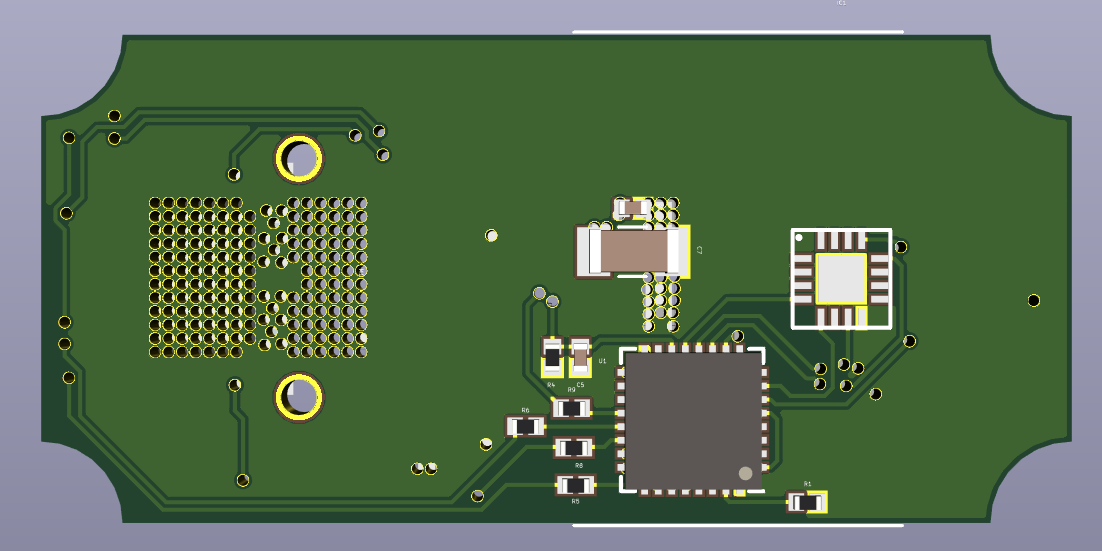
\includegraphics[width=0.6\textwidth]{figures/MotorControllerBottom.png}
       \caption{Motor controller PCB bottom}
       \label{fig:MotortControllerPCBBottom}
   \end{figure}
   \begin{figure}[H]
       \centering
       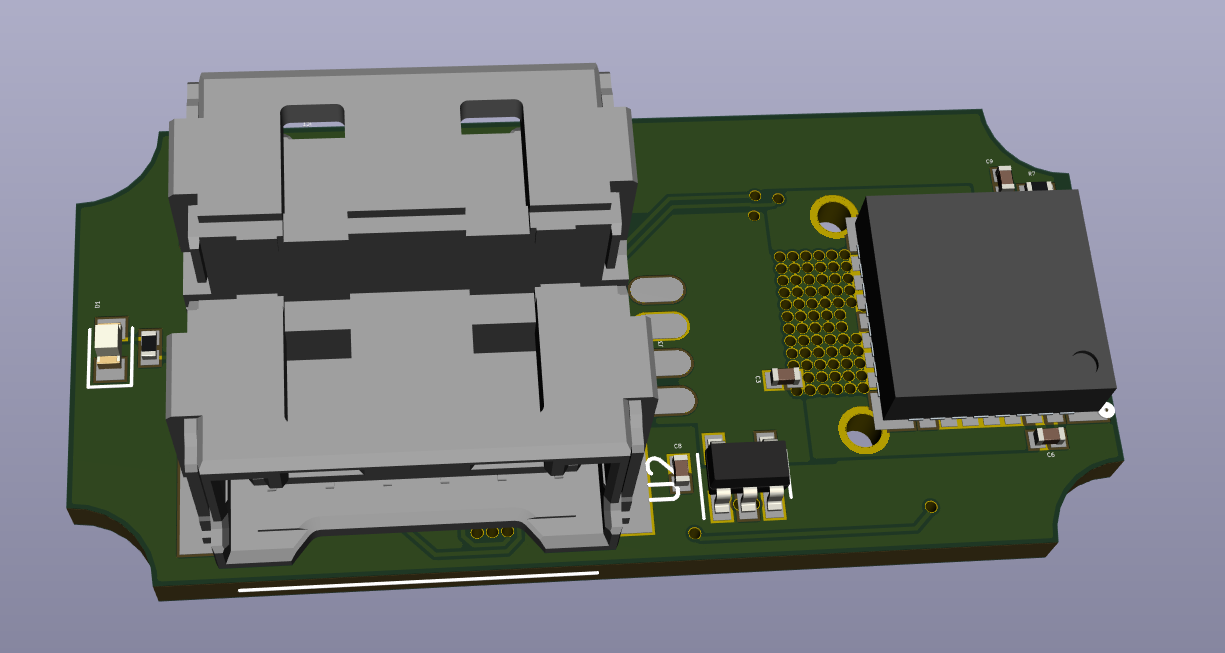
\includegraphics[width=0.6\textwidth]{figures/MotorControllerTop.png}
       \caption{Motor controller PCB top}
       \label{fig:MotorControllerPCBTop}
   \end{figure}
The boards were designed to be assembled directly into the motor connected directly by the motor pins, aligning the encoder above the magnet connected directly to the output shaft of the motor. The programming header was designed as a series of pads that can be used in combination with a pogo pin programming jig, meaning that the firmware can be updated quickly and easily. 
\subsection{Motherboard}
The mother board was developed to be a stand alone micro controller using the STM32H743vit6 micro controller running at 400 MHz. Broken out from this micro controller were all 6 SPI channels, 12 GPIO pins, UART, USB HS and a programming header. In order to limit the number of traces interfering with the High power  coming from the battery, 3.3v and the Ground Plane a 4 layer board was chosen despite the increased cost of production. This meant that all the signal traces could be run internally allowing for a continuous trace running around the periphery of the board connecting all of the connectors to the 8.4v supply coming in from the battery.
\begin{figure}[H]
       \centering
       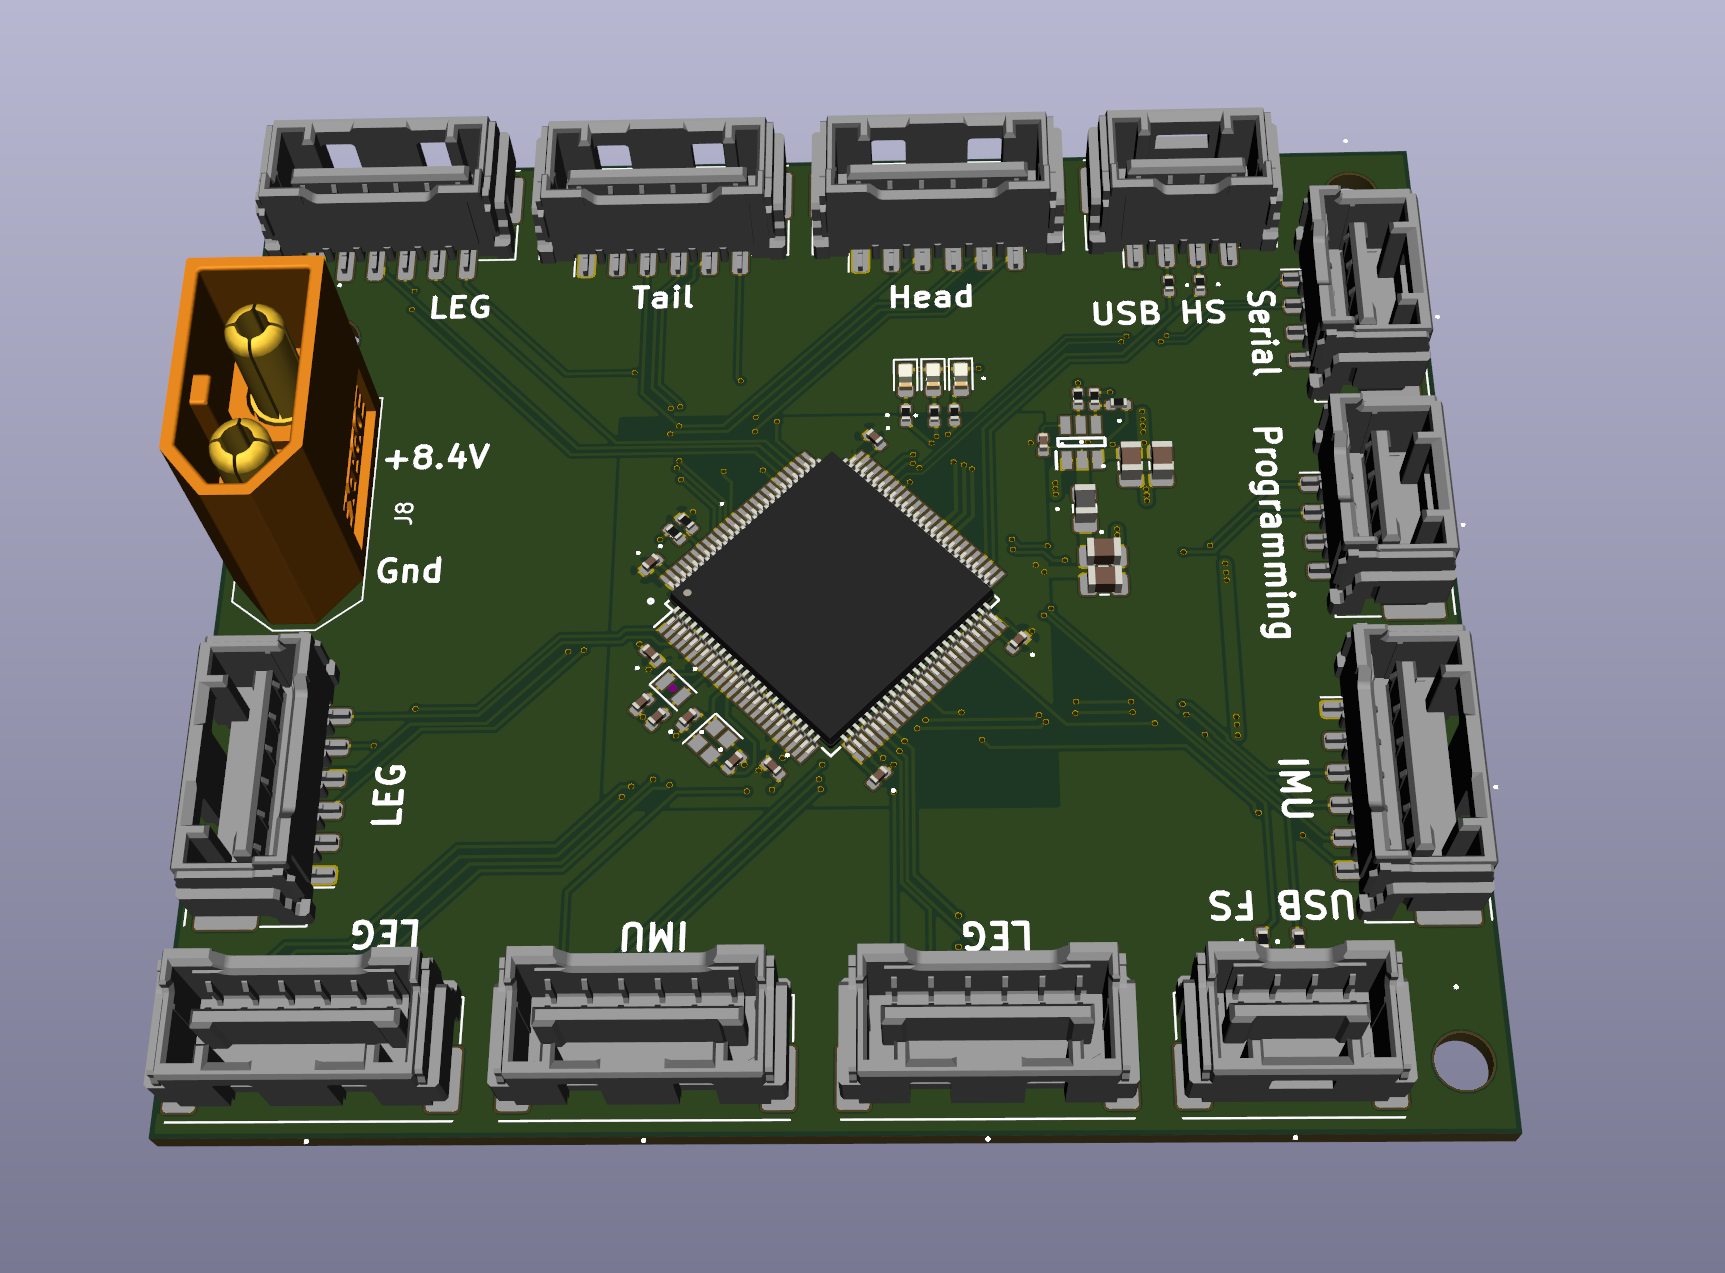
\includegraphics[width=0.6\textwidth]{figures/Motherboard_Rev2.png}
       \caption{Motherboard}
       \label{fig:MotherboardPCB}
   \end{figure}
To ensure reliability at higher clock speeds both a 32.768 kHz crystal oscillator and a 32MHz crystal oscillator were used. While developing the firmware for the motherboard the the clock speed was reduced from 400MHZ to 384 MHz in order to optimize the speed at which the SPI could be run as a clock divisible by 24MHz was requires to take full advantage of the SPI communication with the micro controllers on the motors. In order to have a reliable and stable 3.3v rail for the micro controller, 2 switch mode buck converter power supplies were used in order to stop regulate the 5v supply from USB and the 8.4v supply from the battery pack. This allows the board to be developed on and tested using only power from the USB connection and does not require the battery be connected. 
  
   The motherboard was designed and went through one minor and one major, the minor revision was done to remedy an error in the switch mode power supply circuit as well as to change from USB FS to USB HS allowing for a much faster data  through put at up to 48Mb/s.
 	The Major revision was done in order to switch micro controllers to a micro controller package much better suited for the application. Instead of using the 176 pin package of micro controller, the 100 pin variant was capable of performaing the same tasks required. In addition to the change in micro controller, Both available USB ports were broken out and much more safe guarding against inductive spikes affecting the master microcontroller were implimented due to the death of 2 of the previous revision. Thhough many of these changes were very beneficial, the changing of mincrocontrollers came with a single draw back, the loss of 1 SPI channel, meaning some motors were forces to share SPI channels with other devices on therobot. This prevented us offloading the processing of SPI data to the hardware DMA as it had the possibility of cross talk between multiple devices. The breaking out of both USB ports did allow us to take advantage of the processing power and speed of the micro controller. By combining both ports we were effectively able to double our throughput, sending data and requests for different devices through different ports. Using the USB HS ports for motor data and the USB FS port primarily for IMU data requests allowed us to remove the bottle neck of havinf to wait for the data transmission to be completed and allowed us to increase the sample rate of the IMU.
\subsection{IMU}
\begin{figure}[H]
       \centering
       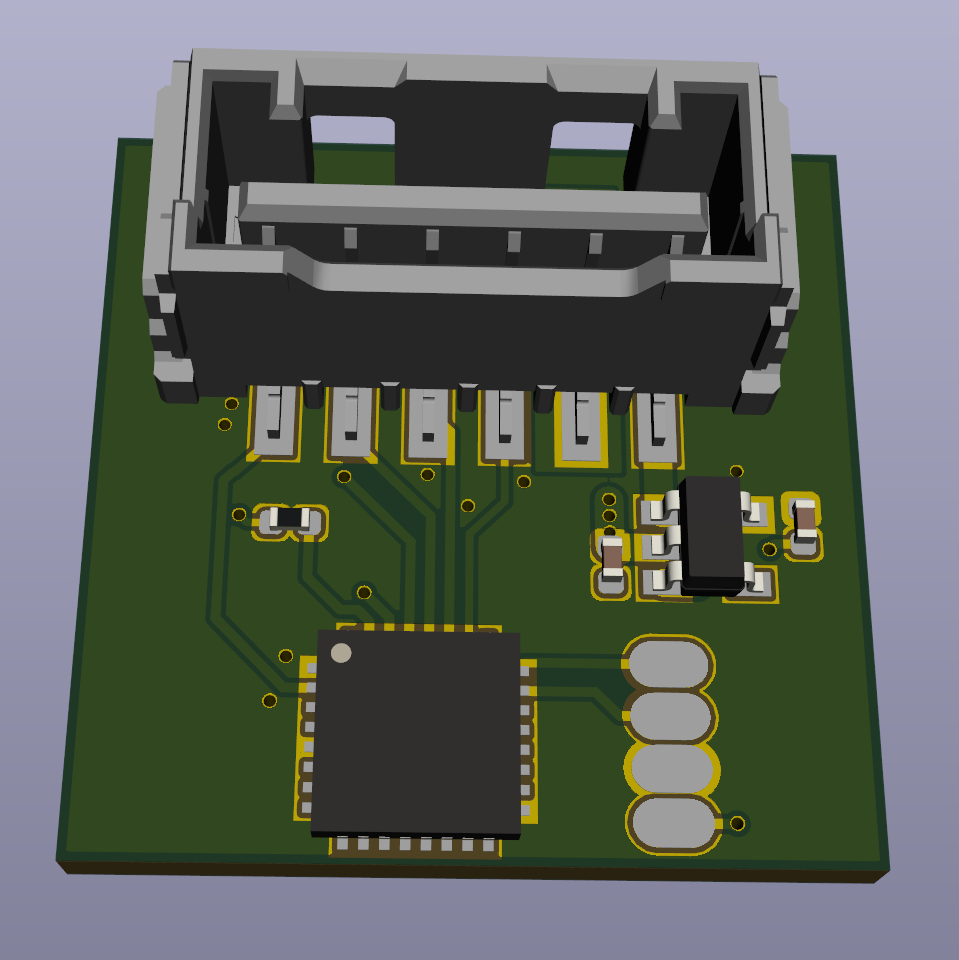
\includegraphics[width=0.6\textwidth]{figures/IMU.png}
       \caption{IMU Breakout}
       \label{fig:IMUPCB}
   \end{figure}
   The IMU breakout allows a BNO055 IMU to be used as any other device in the system, Using the same communication protocol and simular command IDs as the motors, charger, tail controller and other boards in the system. The board continuously samples the BNO055 IMU for Accelerometer, Gyroscope and Euler angles for heading, roll and pitch and on a request for data responds with all 9 of these data sets from the most recent update.This reduses the data request time for the master controller drastically as this IMU is notorious for clock smeering on i2c and having long delays between samples.
   
\subsection{Foot Sensors}
\begin{figure}[H]
       \centering
       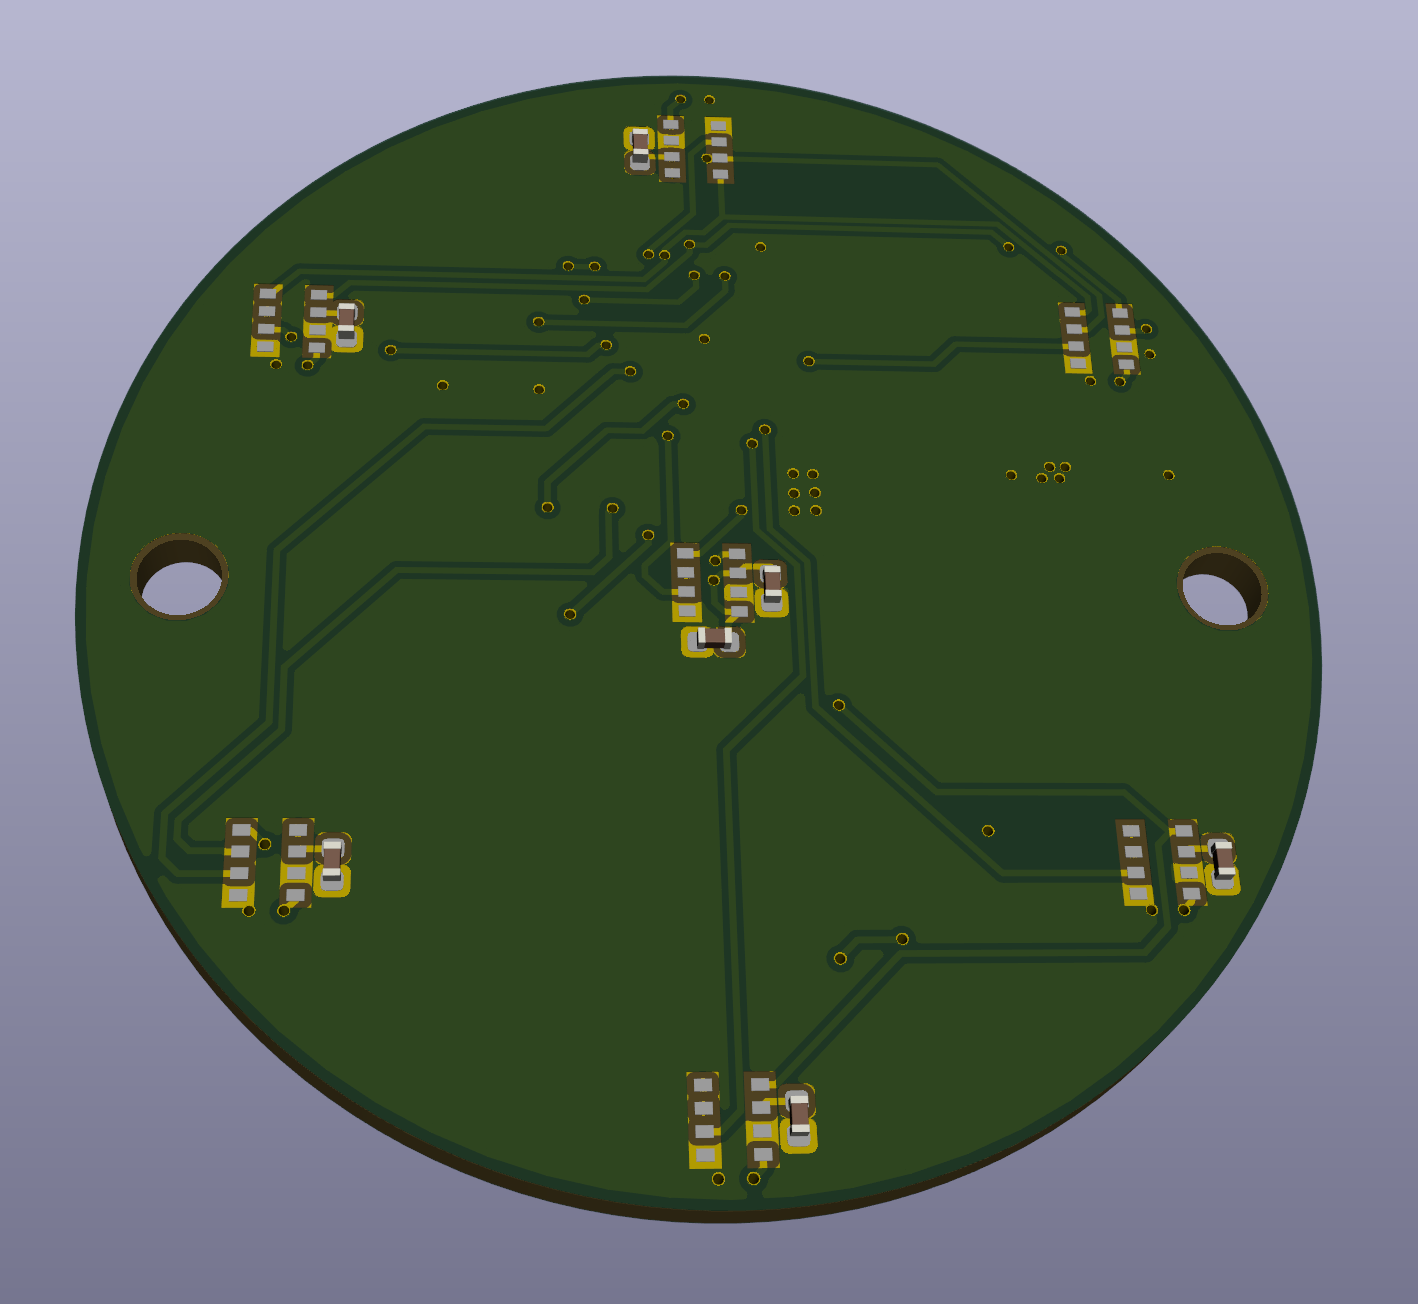
\includegraphics[width=0.6\textwidth]{figures/FootSensor.png}
       \caption{Foot Sensor}
       \label{fig:FootSensorPCB}
   \end{figure}
\subsubsection{Board Design}
\subsubsection{Vector Triangulation}
Many means of calculating the location of the pressure vector were considered however many of them were unreliable and/or difficult to implement on a micro controller using C/C++. This led us to developing a triangulation algorithm similar to that used by police to triangulate a cell phone based on near by cell towers. The pressure of the sensors in a quadrant(one sector of the total sensor) is read and the equations of 3 circles with pressure dependent radius are calculated, the higher the pressure read the smaller the radius of the circle. The intersection points of the circles are then calculated and the equations of 3 lines are found and the intersection point of all three of those is found. This gives the center point of the pressure centroids. 
\begin{figure}[H]
    \centering
    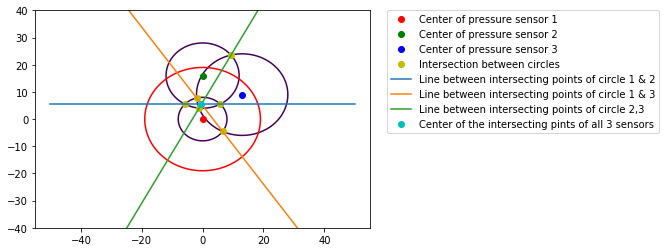
\includegraphics[width=0.8\textwidth]{figures/Triangulation.png}
    \caption{Pressure Vector Triangulation}
    \label{fig:PressureVectorTriangulation}
\end{figure}

\subsection{Charger}
\begin{figure}[H]
       \centering
       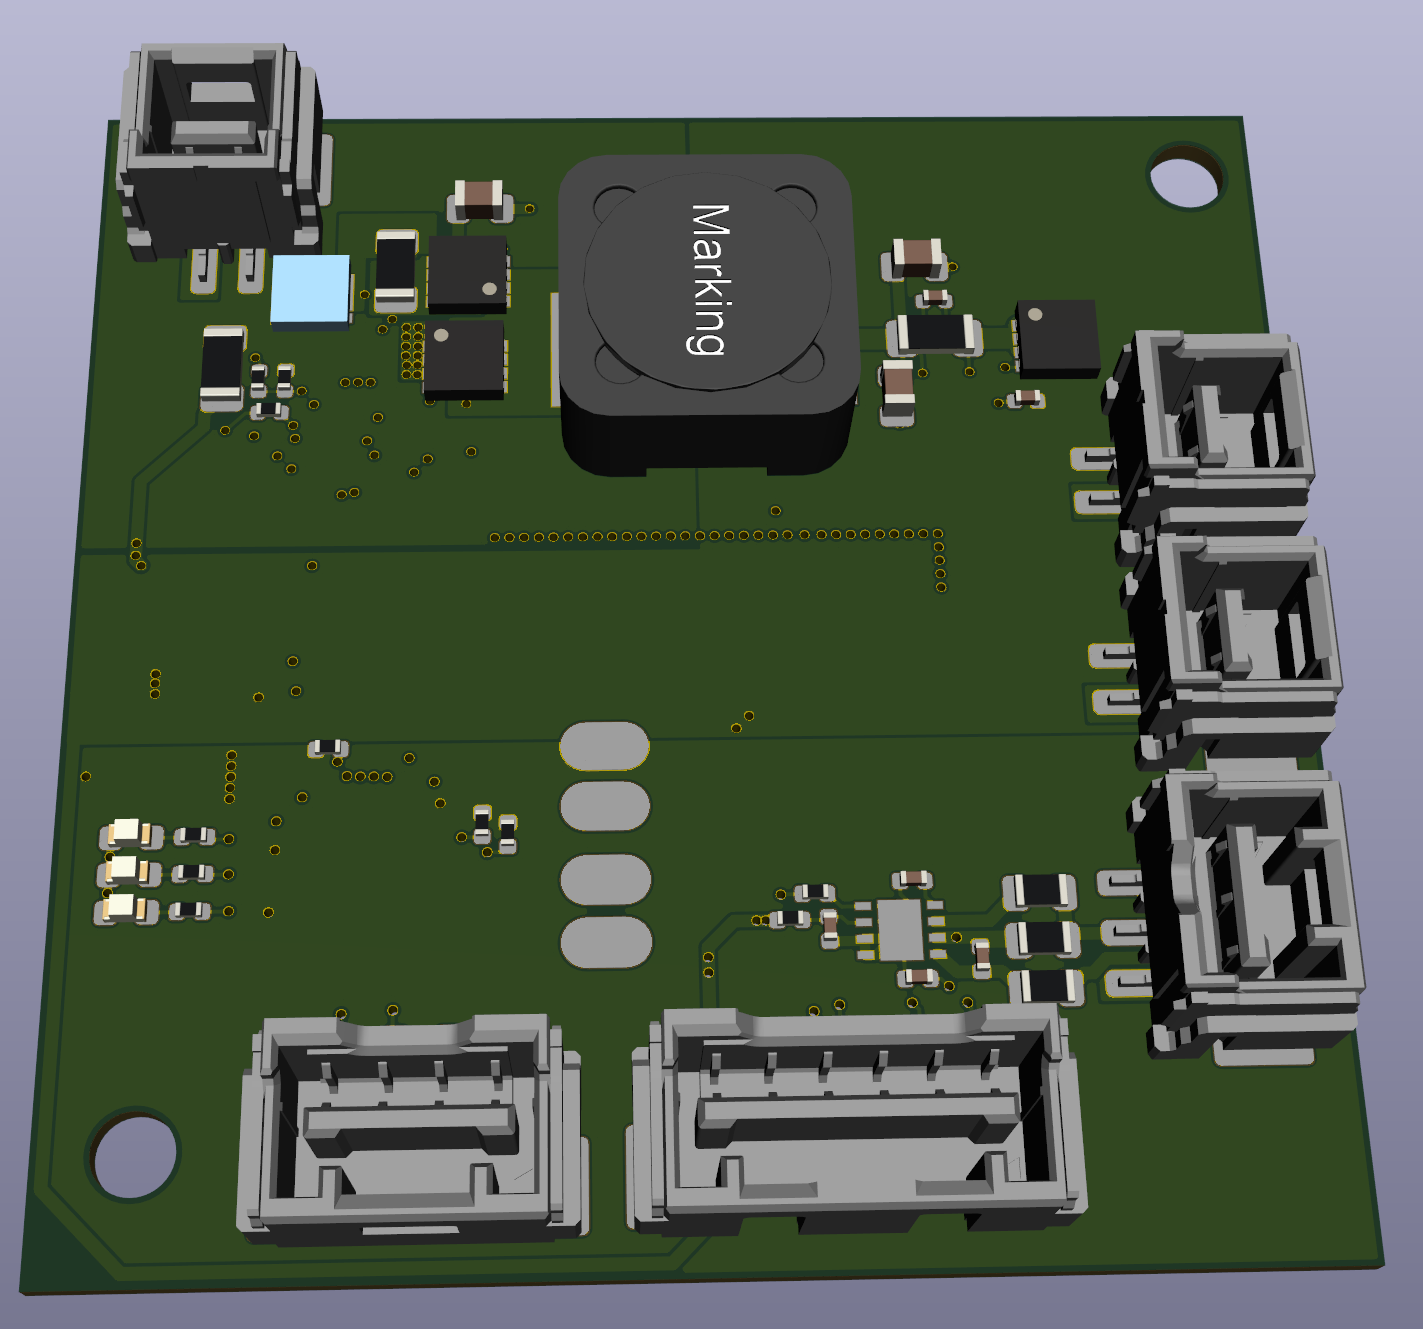
\includegraphics[width=0.6\textwidth]{figures/Charger.png}
       \caption{Battery Charger}
       \label{fig:ChargerPCB}
   \end{figure}


\subsection{Tail Control Board}
\begin{figure}[H]
       \centering
       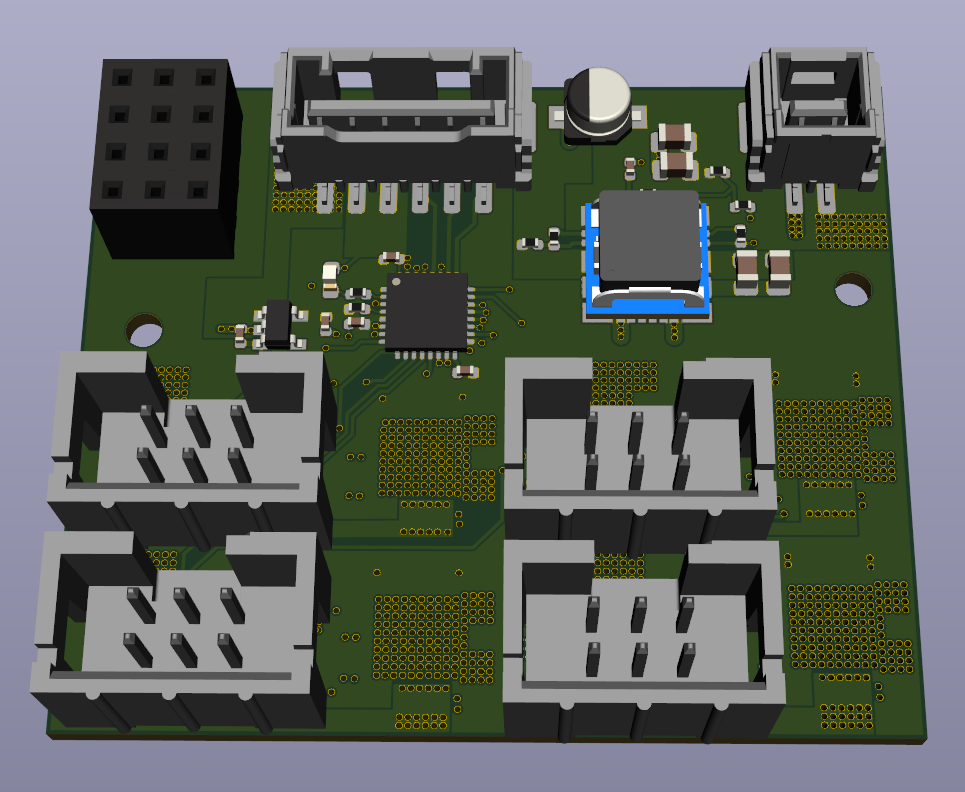
\includegraphics[width=0.6\textwidth]{figures/TailControllerBoard.png}
       \caption{Tail Motor Controller}
       \label{fig:TailControlBoardPCB}
   \end{figure}
   
\subsection{SPI to RS485 Converter Board}
\begin{figure}[H]
       \centering
       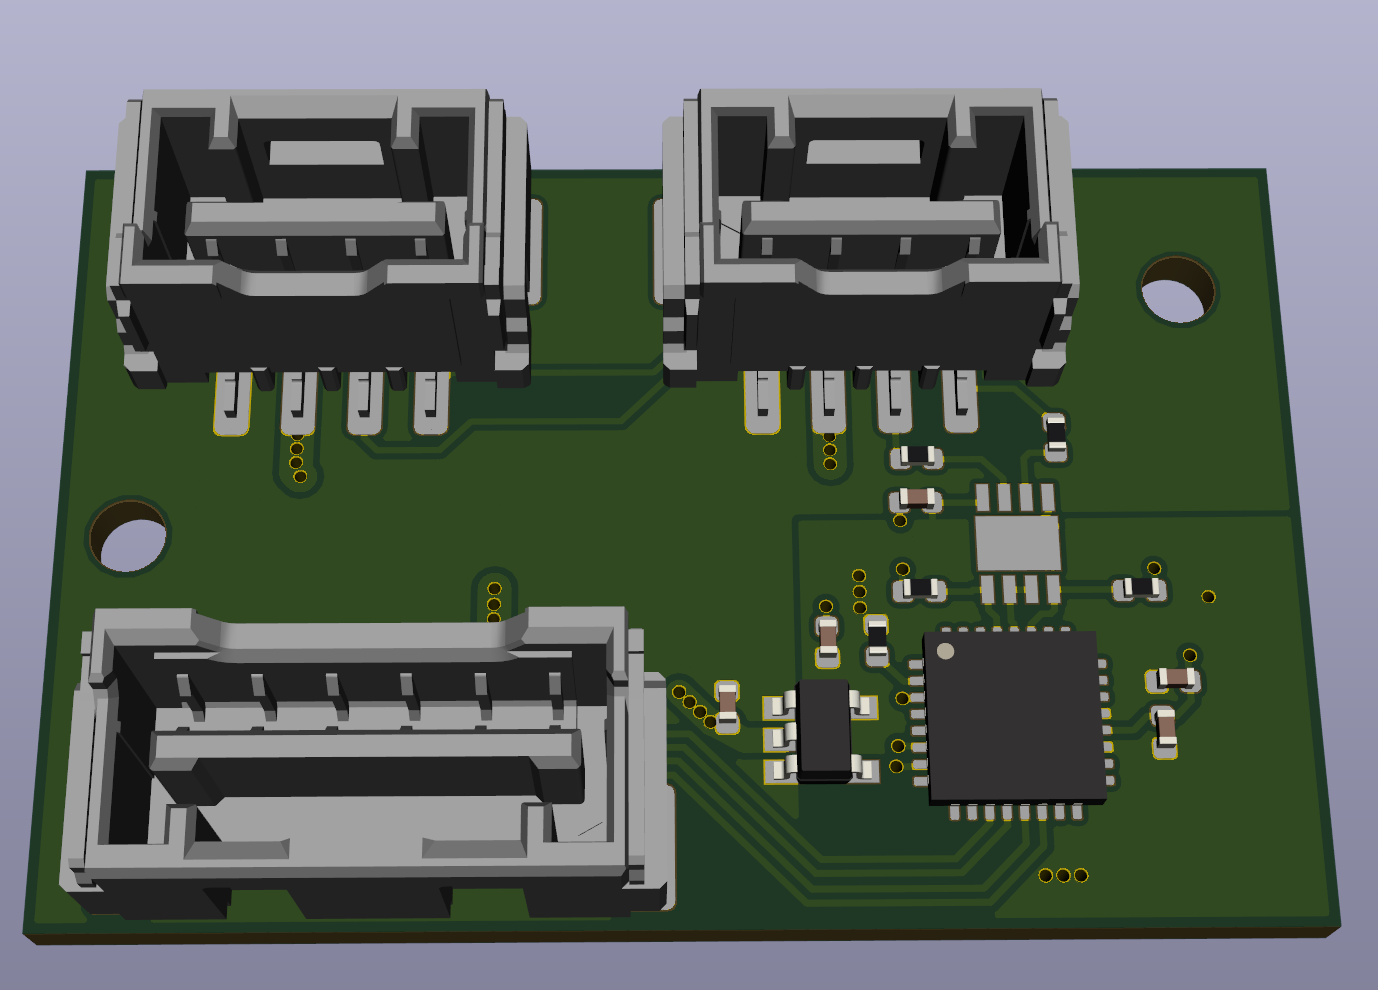
\includegraphics[width=0.6\textwidth]{figures/ConverterBoard.png}
       \caption{SPI to RS485 Converter}
       \label{fig:SPItoRS485ConverterPCB}
   \end{figure}
